% vim:set spell:
% vim:spell spelllang=fr:
\documentclass[a4paper]{article}
\usepackage[utf8x]{inputenc}
\usepackage[T1]{fontenc}
\usepackage{libertine}
\usepackage{helvet}
\usepackage{graphicx}
\usepackage{amsmath,amssymb}
\usepackage[french]{babel}
\usepackage{xspace}
\usepackage{setspace}
\setstretch{1.0}
\usepackage{subfigure}
\usepackage{listings}
\voffset       -1in
\hoffset       -1in
\headheight     12pt
\headsep        12pt
\topmargin      25mm
\oddsidemargin  20mm
\textwidth      170mm
\textheight     240mm
\flushbottom
\lstset{numbers=left, numberstyle=\tiny, stepnumber=1, numbersep=5pt}
\graphicspath{{../../scripts/}}
\begin{document}
\begin{center}
\large
Travaux Pratiques Archi SLE-3A\\
\LARGE
Prédicteur Global de branchements\\
\large

\end{center}
\section{Identification}
Travail réalisé par Damien Cathrine

\section{Prédicteur Global : conception et résultats}
\subsection{Conception}
Le prédicteur implémenté est le prédicteur global utilisant un historique.
La longueur de l'historique est fixée par le premier paramètre donné au simulateur.
L'historique est réalisé avec un entier et un masque. La valeur de cet historique sert
ensuite à accèder aux valeurs (TAKEN ou NOT-TAKEN) enregistrée dans un tableau.

Pour prédire un branchement, on consulte la valeur de la table à l'adresse
\textit{historique} qui nous donne la prédiction.

Lors de la mise à jour, la valeur actuelle du branchement est mise à jour avec l'historique actuel.
Puis l'historique est décalé de la valeur actuelle du branchement.

\subsection{Résultats}
Les résultats issus de la simulation sont les suivants,
\texttt{table size} représente la longueur de l'historique.
\par
\begin{minipage}{.48\linewidth}
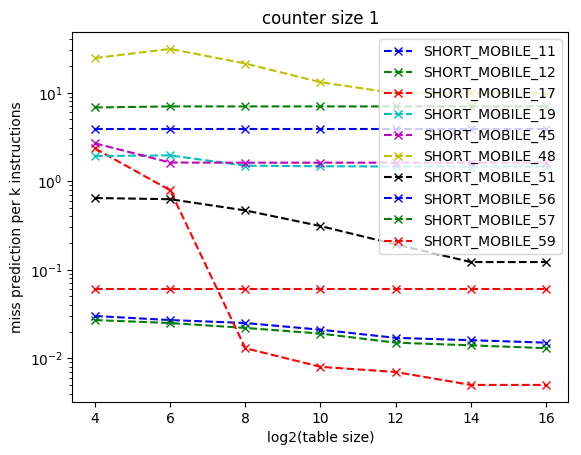
\includegraphics[width=\linewidth]{graph_1}
\end{minipage}%

\subsection{Analyse}
On voit qu'il est utile pour certains test d'avoir un historique plus long.
Cependant pour d'autre, la longueur ne change rien, utiliser un deuxième prédicteur
en parallèle pourrait alors s'avèrer utile.
\end{document}
